\maketitle
\tableofcontents
\newpage

\section{Zielsetzung}
Ziel des Versuches ist es, den Transport von Wärmeenergie entgegen der Richtung des Wärmeflusses
zu untersuchen. Wichtige dabei zu beachtende Größen sind die Güteziffer, der Massendurchsatz und
die mechanische Leistung des Kompressors.
\section{Theorie}
Die Wärmeenergie in einem abgeschlossenen System fließt von der warmen Umgebung in die kalte
Umgebung. Um diesen Wärmefluss umzudrehen, muss mechanische Arbeit erbracht werden. So
eine Maschine wird als Wärmepumpe bezeichnet. Aus dem ersten Hauptsatz der Thermodynamik kommt
\begin{equation}
    \symup{Q_1 = Q_2 + A}
    \label{eqn:3}
\end{equation}
Das Verhältnis zwischen transportierter Wärmemenge und aufgewendeter Arbeit ist definiert
als Güteziffer $\nu$
\begin{equation}
    \nu = \symup{\frac{Q_1}{A}}
    \label{eqn:4}
\end{equation}
Dabei ist A die aufgewendetet Arbeit und $\symup Q_1$ die an das wärmere Reservoir abgegebene
Wärmemenge. Es gilt zu beachten, dass dies die Güteziffer für idealisierte Bedingungen darstellt.
Eine weitere idealisierte Annahme kommt aus dem zweiten Hauptsatz der Thermodynamik
\begin{equation}
    \symup{\frac{Q_1}{T_1} - \frac{Q_2}{T_2}} = 0
    \label{eqn:5}
\end{equation}
Da die Wärmepumpe nicht reversibel arbeiten kann, gilt für die reale Beziehung
\begin{equation}
  \symup{\frac{Q_1}{T_1} - \frac{Q_2}{T_2}} > 0
  \label{eqn:6}
\end{equation}
Nun ergibt sich für \eqref{eqn:4} aus \eqref{eqn:5} und \eqref{eqn:6}
\begin{equation}
  \begin{split}
    \nu_{\symup{ideal}} = \symup{\frac{T_1}{T_1 - T_2}} \\
    \nu_{\symup{real}} < \symup{\frac{T_1}{T_1 - T_2}}
    \label{eqn:7}
  \end{split}
\end{equation}
Aus den Messwerten der Temperaturen gegen die Zeit gewinnt man die später genutzte Formel
für die Berechnung der realen Güteziffer
\begin{equation}
    \nu = \frac{\symup dQ_1}{\symup dt N} = (m_1c_w + m_kc_k) \frac{\symup dT_1}{\symup dt \, N}
    \label{eqn:8}
\end{equation}
mit $m_1c_w$ als Wärmekapazität des Wassers in Reservoir 1, $m_kc_k$ als Wärmekapazität
der Kupferschlange und des Behälters und N als gemittelte Leistungsaufnahme des Kompressors.
Die nächste zu betrachtende Größe ist der Massendurchsatz $\frac{\symup dm}{\symup dt}$, der
sich über den Differentialquotienten berechnet
\begin{equation}
      \frac{\symup dm}{\symup dt} = (m_2 c_w + m_k c_k) \frac{\symup dT_2}{\symup dt \, L}
      \label{eqn:9}
\end{equation}
mit L als Verdampfungswärme.
Als letztes kommt die Formel für die mechanische Kompressorleistung $\symup N_{mech}$
\begin{equation}
    \symup{N_{mech}} = \frac{1}{\kappa - 1} \left(p_b\sqrt[\kappa]{\frac{p_a}{p_b}} - p_a \right) \frac{1}{\rho}
    \frac{\symup dm}{\symup dt}
    \label{eqn:10}
\end{equation}
mit $\kappa$ als Verhältnis der Molwärmen und $\rho$ als Dichte des Gases.
\section{Durchführung}
\subsection{Versuchsaufbau}
Der Versuchsaufbau, siehe \ref{fig:1}, besteht aus den beiden thermisch isolierten Reservoiren, deren Temperatur über zwei
digitale Termometer abgegriffen werden. Zwei Rührmotoren sorgen für die gleichmäßige Durchmischung des Wassers.
Der Drücke $\symup P_a$ und $\symup P_b$ lassen sich an zwei Manometern ablesen. Ein Kompressor
mit angeschlossenem Motor stellt die benötigte mechanische Arbeit A bereit; die aufgewendete Leistung zeigt
ein Wattmeter an. Somit lassen sich alle zu messenden Größen erfassen.
\begin{figure}
  \centering
  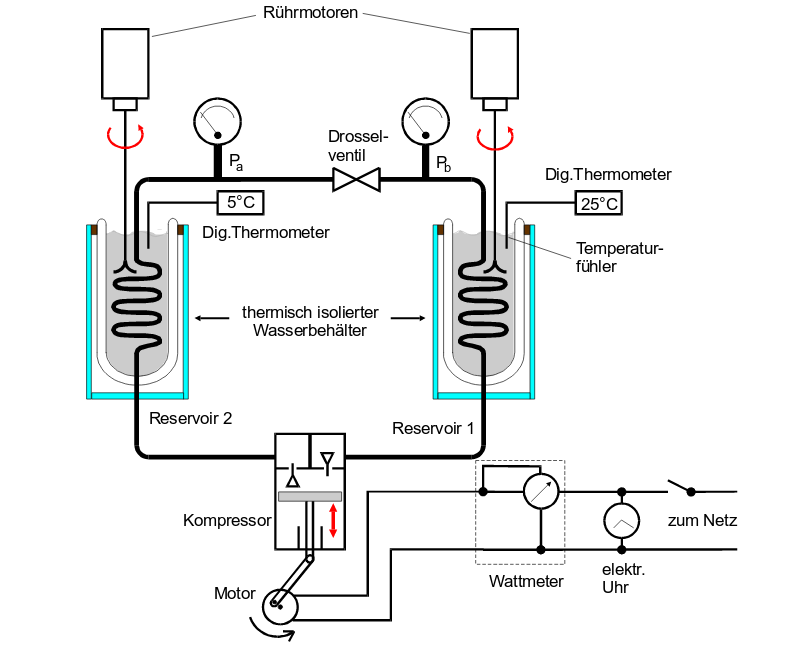
\includegraphics[scale=0.5]{schema.png}
  \caption{Schematische Darstellung des Versuchsaufbaus.}
  \label{fig:1}
\end{figure}
\subsection{Versuchsdurchführung}
Nachdem die Reservoire mit jeweils 3\,$\si{\litre}$ Wasser aufgefüllt wurden,
werden zu Beginn der Messung  die Temperaturen, die Drücke und die Leistung gemessen.
Im $\SI{60}{\second}$ Intervall müssen die oben genannten Größen erfasst werden, bis
$\symup{T_1}$ ungefähr $\SI{50}{\celsius}$ erreicht hat.
\begin{figure}
  \centering
  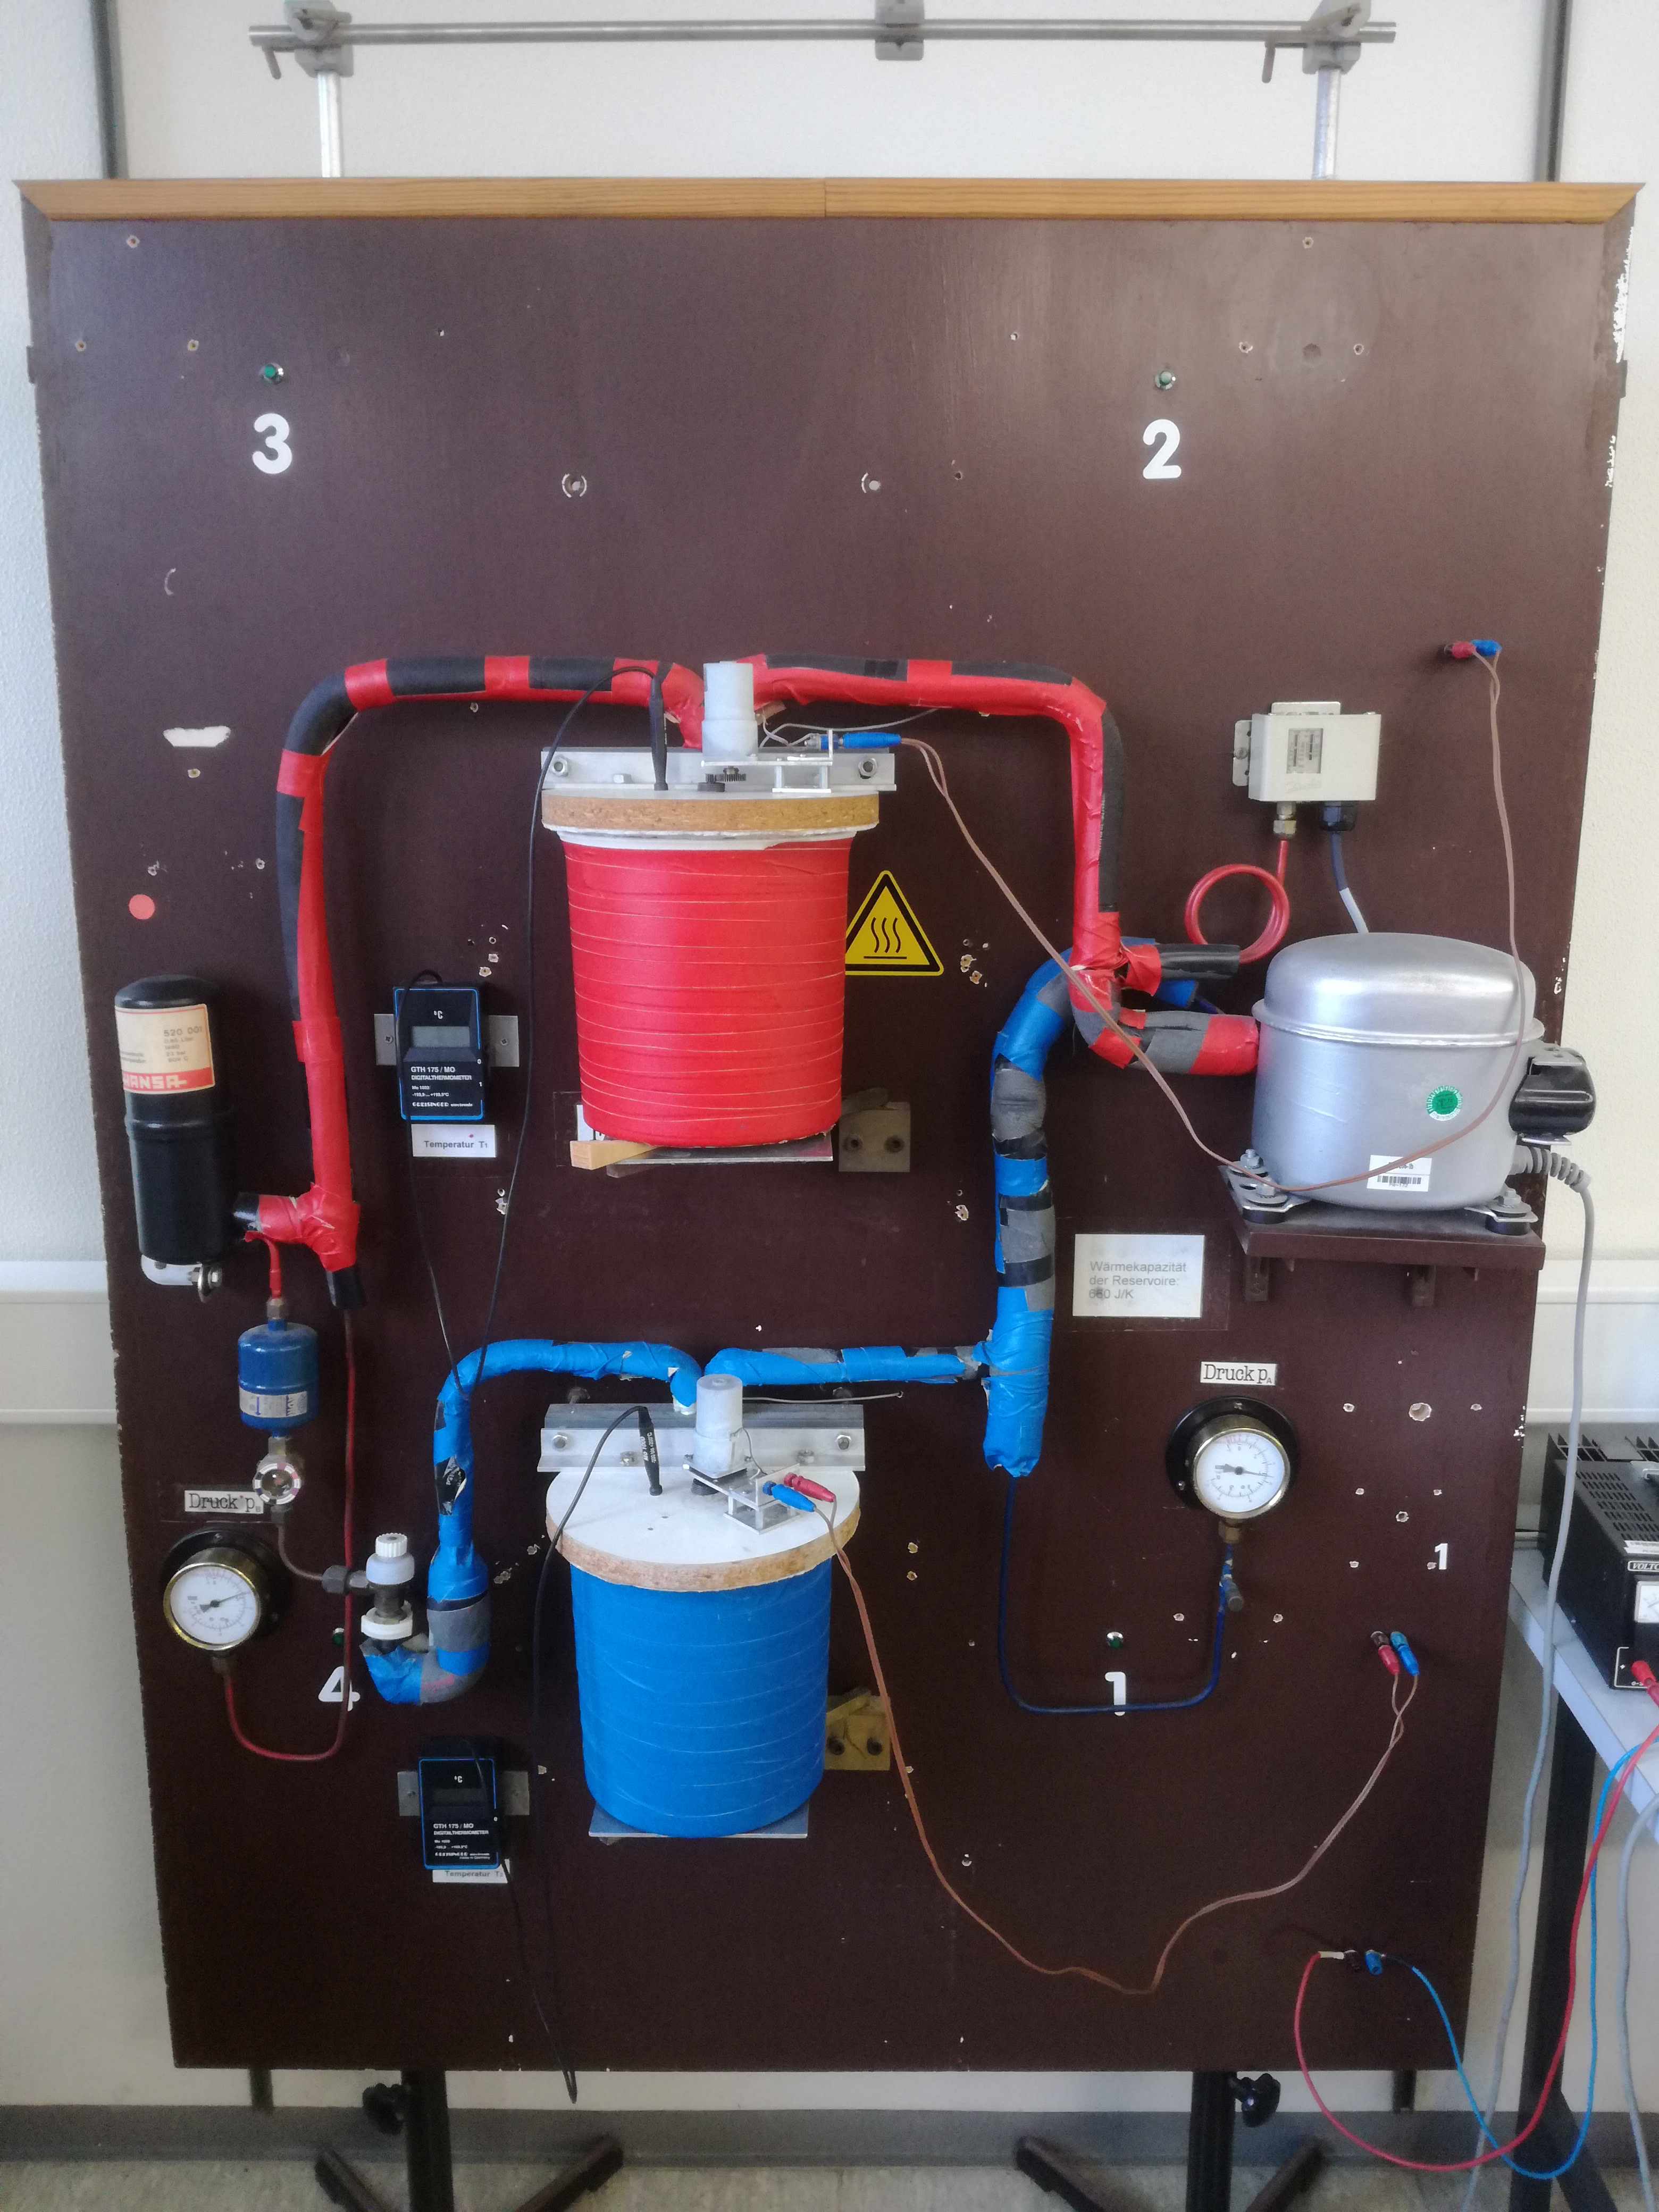
\includegraphics[scale=0.07]{foto.jpg}
  \caption{Der Versuchsaufbau im Foto.}
  \label{fig:2}
\end{figure}
\section{Fehlerrechnung}
Es gibt:
\begin{equation}
  \bar{T} = \frac{1}{n} \sum_{i=1}^{n} T_{i}
  \label{eqn:1}
\end{equation}
den Mittelwert und:
\begin{equation}
  \sigma_{\bar{T}} = \sqrt{\frac{1}{n(n-1)} \sum_{i=1}^{n}(\bar{T}-T_i)^2}
  \label{eqn:2}
\end{equation}
den Fehler des Mittelwertes. Falls zwei fehlerbehaftete Größen in einer Gleichung
zur Bestimmung einer anderen Größe Verwendung finden, dann berechnte sich der Gesamtfehler
nach der Gaußschen Fehlerfortpflanzung zu
\begin{equation}
    \symup \Delta f(x_1, x_2, ..., x_n) = \sqrt{\left(\frac{\symup df}{\symup dx_1} \symup \Delta
    x_1 \right)^2 +    \left(\frac{\symup df}{\symup dx_2} \symup \Delta
    x_2 \right)^2 + ... + \left(\frac{\symup df}{\symup dx_n} \symup \Delta x_n \right)^2} \ .
\end{equation}

\section{Auswertung}
\begin{figure}[p]
  \centering
  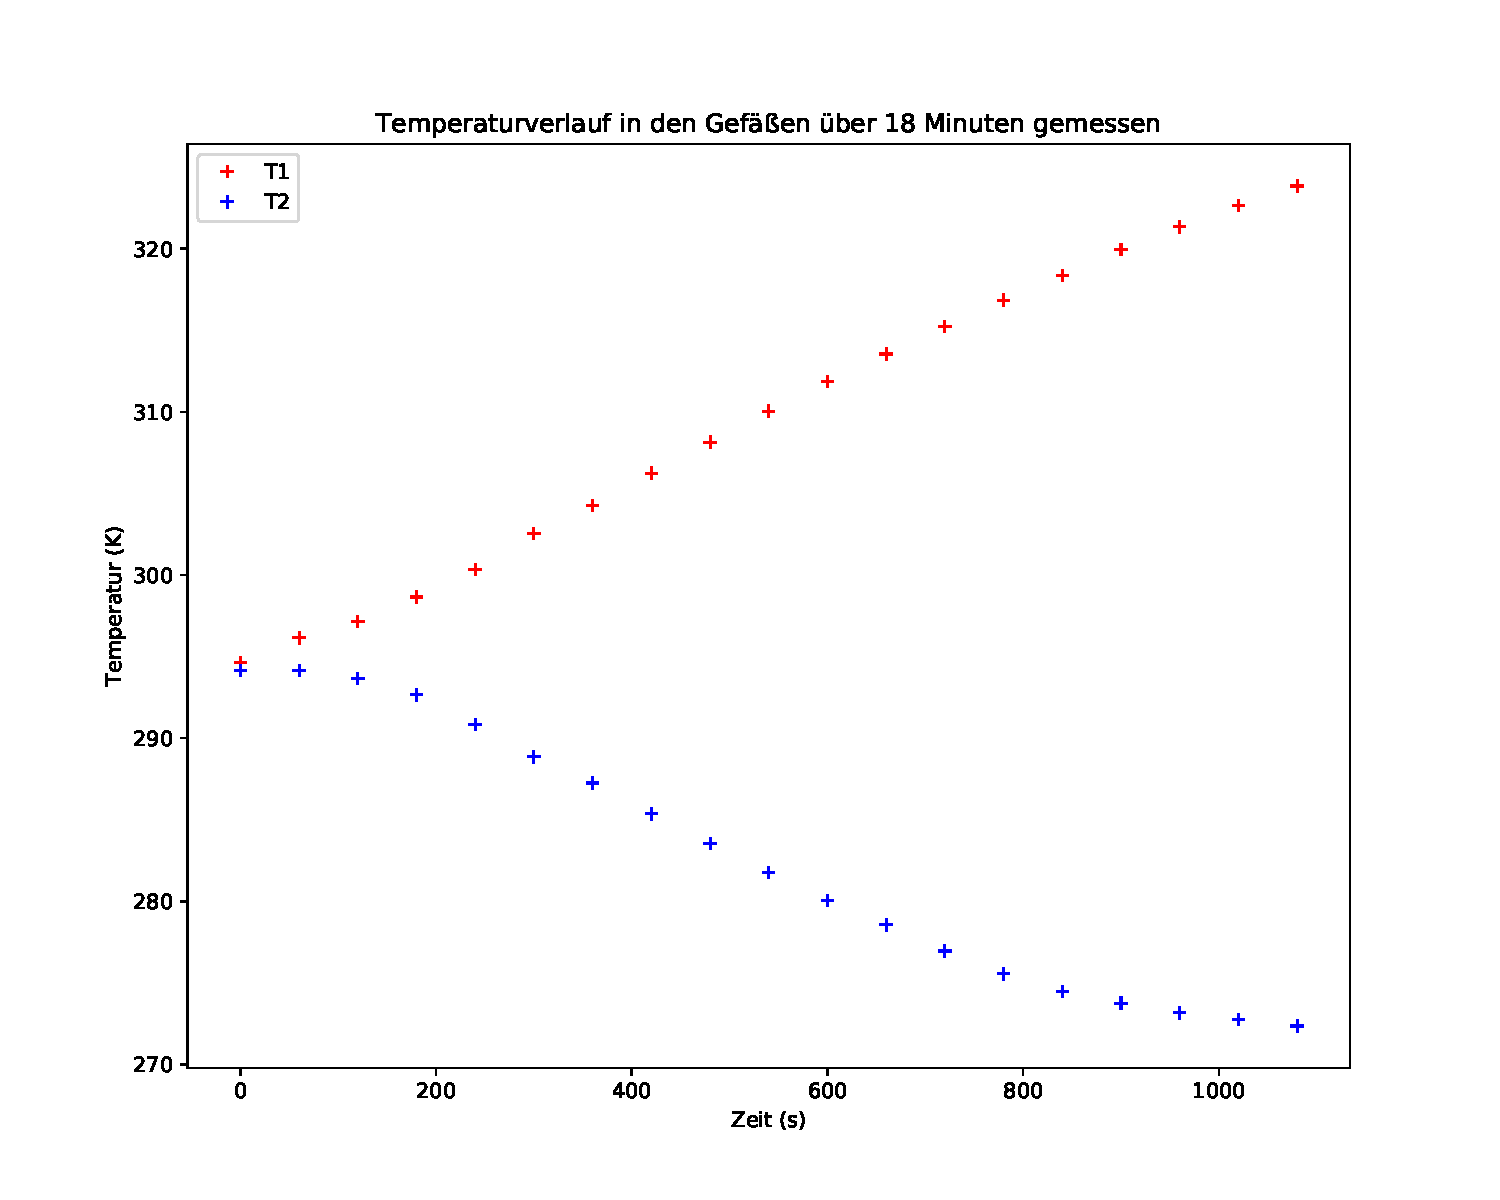
\includegraphics[width=\textwidth]{verlauf.pdf}
  \caption{Temperaturverlauf ohne Regression.}
  \label{fig:5}
\end{figure}
\label{sec:Auswertung}
\begin{figure}[p]
  \centering
  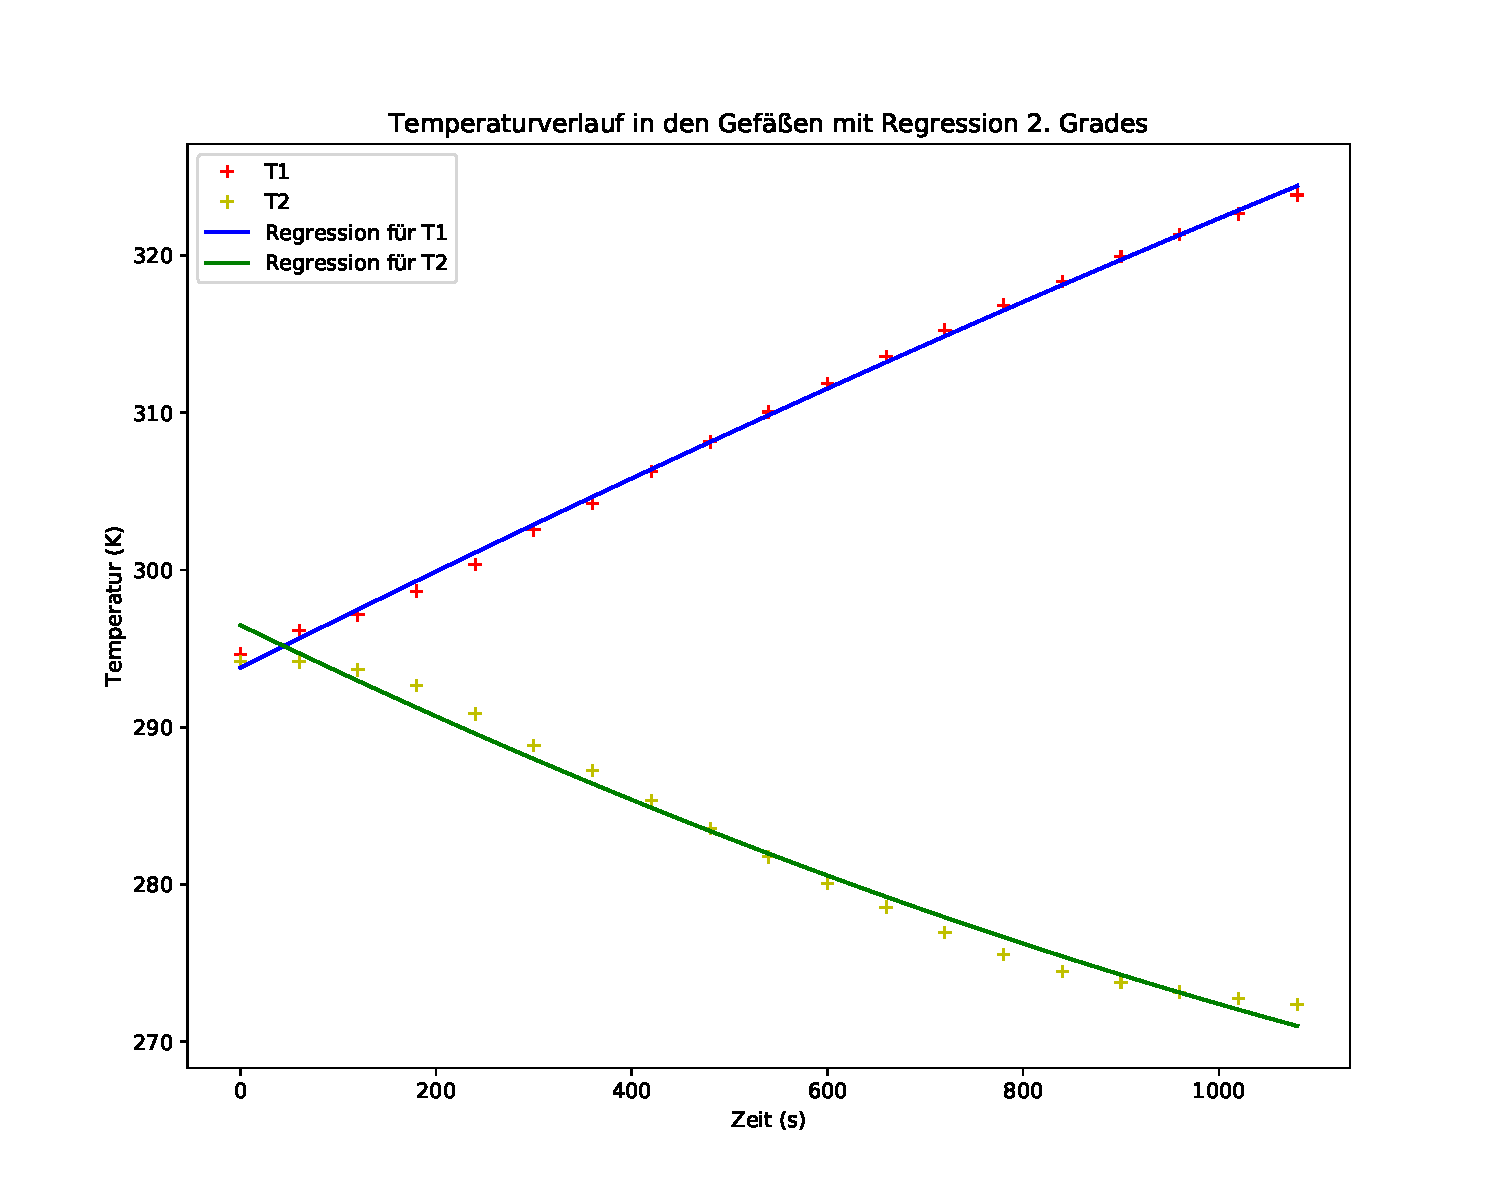
\includegraphics[width=\textwidth]{Grad2.pdf}
  \caption{Temperaturverlauf durch $T(t) = At^2 + Bt + C$ approximiert.}
  \label{fig:3}
\end{figure}
Die Regression mit einer Funktion zweiten Grades, siehe \ref{fig:3} ist, vor
allem für die Werte von $T_2$, ungeeignet als Aproximation. Es folgen die in \ref{tab:7} dargestellten Koeefizienten.
\begin{table}
  \centering
  \caption{Parameter für Ansatz $T(t) = At^2 + Bt + C$, siehe  \ref{fig:3}.}
  \label{tab:7}
  \begin{tabular}{c c c}
    \toprule
    Parameter & $\symup{T_1}$ & $\symup{T_2}$ \\
    \midrule
    A & \SI{-2.6(11)e-6}{\kelvin\per\second\squared} & \SI{6.1(25)e-6}{\kelvin\per\second\squared} \\
    B & \SI{0.031(1)}{\kelvin\per\second} & \SI{-0.030(3)}{\kelvin\per\second} \\
    C & \SI{293.8(3)}{\kelvin} & \SI{296.5(7)}{\kelvin} \\
    \bottomrule
  \end{tabular}
\end{table}
Eine bessere Annäherung erhält man für eine Funktion mit Grad 3, siehe \ref{fig:4}.
Mit diesem Ansatz ist eine vertretbare Approximation gefunden. Die Koeefizienten für diesen Ansatz finden sich in \ref{tab:1}
\\
\\
Die orginalen Messdaten finden sich in Tabelle \ref{tab:6} wieder. Die Drücke
$p_a$ und $p_b$ enthalten bereits den Normaldruck von $\SI{1}{\bar}$ . Die Temperaturen
wurden für alle folgenden Rechnungen in $\si{\kelvin}$, die Zeiten in $\si{\second}$ und die Drücke in $\si{\pascal}$ umgewandelt.
\begin{table}
  \centering
  % Bessere caption?
  \caption{Minütlich gemessene Temperaturen, Drücke und Leistung des Versuchs.}
  \label{tab:6}
  \begin{tabular}{c c c c c c}
    \toprule
    Zeit/$\si{\minute}$ & $T_1$/$\si{\celsius}$ & $p_b$/$\si{\bar}$ &
    $T_2$/$\si{\celsius}$ & $p_a$/$\si{\bar}$ & N/$\si{\watt}$ \\
    \midrule
    0 & 21.5 & 5.25 & 21 & 5 & 0 \\
    1 & 23 & 7 & 21 & 2.6 & 170 \\
    2 & 24 & 7.5 & 20.5 & 2.8 & 180 \\
    3 & 25.5 & 7.5 & 19.5 & 3 & 190 \\
    4 & 27.2 & 8 & 17.7 & 3.2 & 197 \\
    5 & 29.4 & 8.25 & 15.7 & 3.2 & 200 \\
    6 & 31.1 & 8.75 & 14.1 & 3.2 & 204 \\
    7 & 33.1 & 9 & 12.2 & 3.2 & 205 \\
    8 & 35 & 9.5 & 10.4 & 3.2 & 206 \\
    9  & 36.9 & 10   & 8.6 & 3.2 & 209 \\
    10 & 38.7 & 10.5 & 6.9 & 3.2 & 209 \\
    11 & 40.4 & 11   & 5.4 & 3.2 & 210 \\
    12 & 42.1 & 11.25 & 3.8 & 3.2 & 212 \\
    13 & 43.7 & 11.5 & 2.4 & 3.2 & 212 \\
    14 & 45.2 & 12   & 1.3 & 3.2 & 213 \\
    15 & 46.8 & 12.5 & 0.6 & 3.2 & 211 \\
    16 & 48.2 & 12.75 & 0 & 3.2 & 210 \\
    17 & 49.5 & 13 & -0.4 & 3.2 & 207 \\
    18 & 50.7 & 13.5 & -0.8 & 3.2 & 206 \\
    \bottomrule
  \end{tabular}
\end{table}
\\
\\
Die Parameter bestimmen sich nach Tabelle \ref{tab:1}.
\begin{table}[h]
  \centering
  \caption{Parameter für Ansatz $T(t) = At^3 + Bt^2 + Ct + D$, siehe  \ref{fig:4}.}
  \label{tab:1}
  \begin{tabular}{c c c}
    \toprule
    Parameter & $\symup{T_1}$ & $\symup{T_2}$ \\
    \midrule
    A & \SI{-1.406(165)e-8}{\kelvin\per\cubic\second} & \SI{3.383(269)e-8}{\kelvin\per\cubic\second} \\
    B & \SI{2.022(271)e-5}{\kelvin\per\second\squared} & \SI{-4.869(442)e-5}{\kelvin\per\second\squared} \\
    C & \SI{0.022(1)}{\kelvin\per\second} & \SI{-0.007(2)}{\kelvin\per\second} \\
    D & \SI{0.022(1)}{\kelvin} & \SI{294.704(245)}{\kelvin} \\
    \bottomrule
  \end{tabular}
\end{table}
\begin{figure}[p]
  \centering
  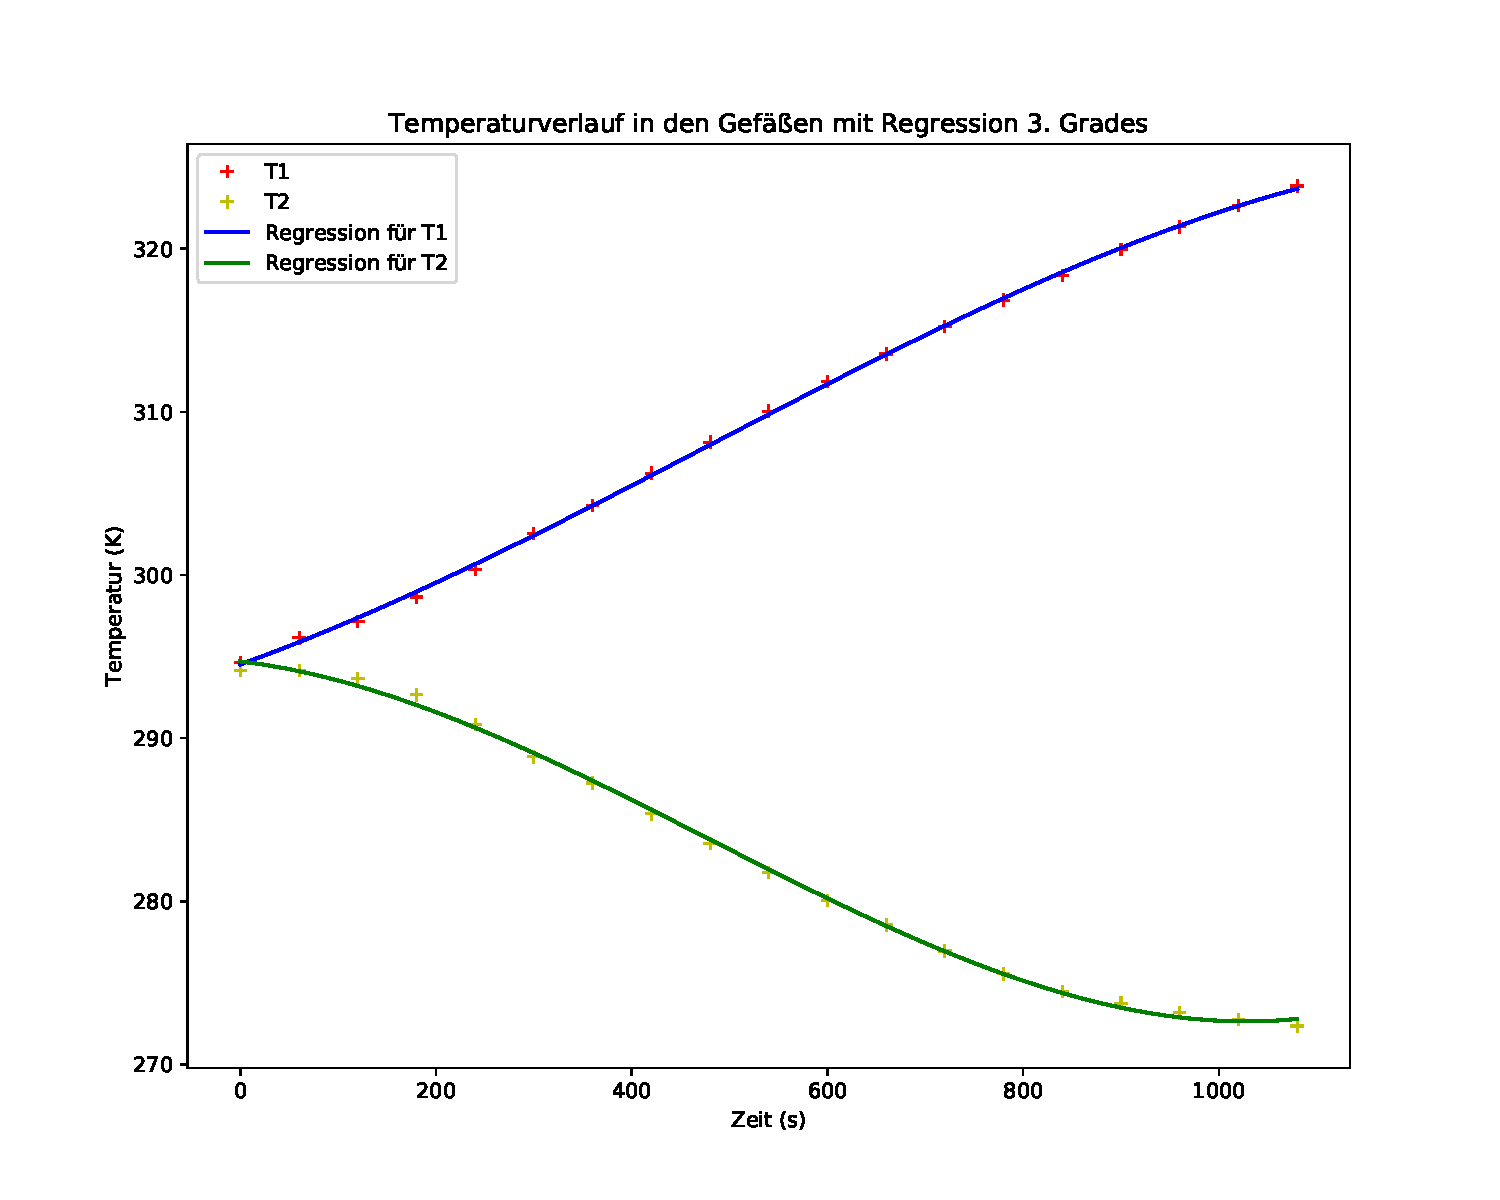
\includegraphics[width=\textwidth]{Grad3.pdf}
  \caption{Temperaturverlauf durch $T(t) = At^3 + Bt^2 + Ct + D$ approximiert.}
  \label{fig:4}
\end{figure}
Für die Differentialqutionten $\frac{\symup dT_1}{\symup dt}$ und $\frac{\symup dT_2}{\symup dt}$
ergeben sich für vier verschiedene Temperaturen zu vier verschiedenen Zeiten
die Werte in Tabelle \ref{tab:2}.
\begin{table}[h]
  \centering
  \caption{Differentialquotienten $\frac{\symup dT_1}{\symup dt}$ und $\frac{\symup dT_2}{\symup dt}$.}
  \label{tab:2}
  \begin{tabular}{c c c}
    \toprule
    Zeit/$\si{\second}$ & $\frac{\symup dT_1}{\symup dt}$/$\si[per-mode=reciprocal]{\kelvin\per\second}$
    & $\frac{\symup dT_2}{\symup dt}$/$\si[per-mode=reciprocal]{\kelvin\per\second}$ \\
    \midrule
    240 & 0.026 \pm 0.001 & -0.017 \pm 0.002 \\
    480 & 0.028 \pm 0.002 & -0.023 \pm 0.003 \\
    720 & 0.029 \pm 0.003 & -0.025 \pm 0.004 \\
    960 & 0.028 \pm 0.003 & -0.023 \pm 0.005 \\
    \bottomrule
  \end{tabular}
\end{table}

\subsection{Bestimmung der Güteziffer}
\label{Güteziffer}
Für die Güteziffer ergibt sich nach Formel \eqref{eqn:8} in Vergleich mit der idealen Güteziffer
nach \eqref{eqn:7} die Werte in Tabelle \ref{tab:3}.
\begin{table}[h]
  \centering
  \caption{Güteziffern der Wärmepumpe für die Zeiten aus \ref{sec:Auswertung}.}
  \label{tab:3}
  \begin{tabular}{c c c}
  \toprule
  Zeit/$\si{\second}$ & $\nu_{\symup{real}}$ & $\nu_{\symup{ideal}}$  \\
  \midrule
  240 & 1.763 \pm 0.097 & 29.998 \pm 2.093 \\
  480 & 1.930 \pm 0.126 & 12.730 \pm 0.882 \\
  720 & 1.985 \pm 0.170 & 8.220 \pm 0.707 \\
  960 & 1.929 \pm 0.224 & 6.622 \pm 0.786 \\
  \bottomrule
  \end{tabular}
\end{table}
Die Wärmekapazität $m_kc_k$ für die Kupferschlange und die Behälter beträgt
$\SI{660}{\joule\per\kelvin}$, die Größe N, also die gemittelte Leistung,
\SI{192.16}{\watt}. Für die spezifische Wärmekapazität $c_w$ ergibt sich nach
\cite{chemie} $\approx \SI{4.19E3}{\joule\per\kilo\gram\per\kelvin}$ mit $m_1 =$
$\SI{3}{\kilo\gram}$.

\subsection{Berechnung des Massendurchsatzes $\frac{\symup dm}{\symup dt}$}
\label{Masse}
Für den Massendurchsatz ergibt sich nach \eqref{eqn:9} die Ergebnisse,
die in Tabelle \ref{tab:4} aufgeführt sind.
\begin{table}[h]
  \centering
  \caption{Massendurchsatz $\frac{\symup dm}{\symup dt}$ für die Zeiten aus \ref{sec:Auswertung}.}
  \label{tab:4}
  \begin{tabular}{c c}
    \toprule
    Zeit/$\si{\second}$ & Massendurchsatz $\frac{\symup dm}{\symup dt}$/$\si[per-mode=reciprocal]{\kilo\gram\per\second}$ \\
    \midrule
    240 & -0.0013 \pm 0.0002 \\
    480 & -0.0018 \pm 0.0003 \\
    720 & -0.0019 \pm 0.0003 \\
    960 & -0.0018 \pm 0.0004 \\
    \bottomrule
  \end{tabular}
\end{table}
Die Addition der Wärmekapazitäten ist vom Wert her gleich wie in \ref{Güteziffer},
da $m_2$ auch $\SI{3}{\kilo\gram}$ beträgt und sich ansonsten nichts geändert hat.
Die Bestimmung von L, der Verdampfungswärme, erfolgt indem man den Druck $p_b$
logarithmisch gegen $\frac{1}{T_1}$ aufträgt über lineare Regression die Steigung bestimmt.
\begin{equation*}
  \begin{split}
%   ln(p_b) = a \frac{1}{T_1} + b
    m = \SI{-2.45(14)}{\kelvin} \\
    b = \SI{10.2(5)}{\bar}
   \label{eqn:11}
 \end{split}
\end{equation*}
Nach der Formel
\begin{equation}
    L = \frac{-R \cdot m}{M}
    \label{eqn:12}
\end{equation}
ergibt sich für L $\SI{1.68 \pm 0.10E5}{\joule\per\kilo\gram}$.
Dabei ist R die allgemeine Gaskonstante \cite{gaskonstante} mit dem Wert
$R = \SI{8.314}{\joule\per\kelvin\per\mol}$
und $M = \SI{120.9E-3}{\kilo\gram\per\mol}$ die molare Masse \cite{molar} des Transportgases.

\subsection{Mechanische Leistung des Kompressors}
Hiefür wird Formel \eqref{eqn:10} genutzt. Da die Dichte aber sowohl druck-
als auch temperaturabhängig ist, errechnet sich $\rho$ nach der allgemeinen
Gasgleichung
\begin{equation}
  \frac{p_0}{\rho_0 \ T_0} = \frac{p_a}{\rho \ T_2} \ .
  \label{eqn:13}
\end{equation}
Umgestellt nach $\rho$ ergibt sich aus \eqref{eqn:13}
\begin{equation}
    \rho = \frac{\rho_0 \ T_0 \ p_a}{p_0 \ T_2} \ .
    \label{eqn:14}
\end{equation}
Mit den im Kapitel \ref{Masse} berechneten Massendurchsätzen, den im Experiment
bestimmten Drücken $p_a \text{und} \ p_b$, $\kappa = 1.14$
\footnote{laut Aufgabenstellung, siehe \cite{anleitung}} sowie den eben errrechneten
Werten für $\rho$ zu den vier Zeitpunkten lässt sich nun die mechanische Kompressorleistung
bestimmen. Der Wirkungsgrad bestimmt sich zu:
\begin{equation}
  \eta = \frac{N_{mech}}{\overline{N}}
\end{equation}
Die Ergebnisse sind in Tabelle \ref{tab:5} dargestellt.
% Quotient aus Nmech und gemittelter Leistung?
\begin{table}[h]
  \centering
  \caption{Der Druck $\rho$, die mechanische Kompressorleistung sowie den Wirkungsgrad für die Zeiten aus \ref{sec:Auswertung}.}
  \label{tab:5}
  \begin{tabular}{c c c c}
    \toprule
    Zeit/$\si{\second}$ & Dichte $\rho$/$(\si[per-mode=reciprocal]{\kilo\gram\per\cubic\meter})$ & $N_{mech}$/$\si{\watt}$ & $\eta/\%$\\
    \midrule
    240 & 16.571 \pm 0.034 & 21.857 \pm 3.174 & 11.4 \pm 1.7\\
    480 & 16.971 \pm 0.087 & 34.479 \pm 4.789 & 17.9 \pm 2.5\\
    720 & 17.392 \pm 0.183 & 42.615 \pm 6.937 & 22.2 \pm 3.6\\
    960 & 17.650 \pm 0.331 & 42.851 \pm 9.538 & 22.3 \pm 5.0\\
    \bottomrule
  \end{tabular}
\end{table}

\section{Diskussion}
Die Werte für die Temperaturen lassen sich am besten mit einer ganzrationalen
Funktion dritten Grades approximieren, was die verschiedenen Graphen deutlich zeigen.
Diese zeigen, dass die Temperatur zu Beginn und zum Ende der Messung relativ langsam
fallen, dagegen in der Mitte der Messung am schnellsten. Dies passt am besten zu der
oben gennanten ganzrationalen Funktion dritten Grades.
\\
\\
Vor allem die Werte der Güteziffer liegen weit außerhalb des Toleranzbereichs
der Fehlergrenzen. Die realen Güteziffern sind für alle Zeiten kleiner als die
idealen. Dies ist unter anderem darauf zurückzuführen, dass die Reservoire nicht
gut isoliert sind und so ein Wärmeaustausch mit der Umgebung stattfinden kann,
da zum Beispiel die Deckel nicht bündig auf den Reservoiren sitzen.
Weiterhin sind die schlecht leitenden Kupferschlangen im Wechselspiel mit einem
ineffizienten Kompressor mögliche Optimierungsmöglichkeiten.
\\
\\
Im Allgemeinen lässt sich sagen, dass die Wärmepumpe wesentlich effizienter arbeiten
könnte als sie es aktuell tut. Insbesondere ein Kompressor mit höherem Wirkungsgrad
sowie eine bessere Abschirmung der Gefäße, besonders nach oben, würden die Effizienz
dieser Wärmepumpe weiter steigern. Als bloßes Modell einer Wärmepumpe ist sie jedoch gut geeignet
und anschaulich zu beschreiben.
\newpage
\nocite{*}
\printbibliography
